\chapter{Implementación}
En este capítulo se va a abordar la implementación del sistema. Para ello, en
primer lugar, se van a explicar las herramientas y tecnologías que se han utilizado
y el porqué de su elección. En segundo lugar, se explicará la implementación de la
base de datos, se mostrará el diagrama de clases y, por último, se explicará la
implementación de la aplicación, tanto del backend como del frontend.

\section{Herramientas y tecnologías}
En este apartado se van a explicar las herramientas y tecnologías utilizadas
para el desarrollo de la aplicación.

\subsection{Control de versiones}
Para realizar un seguimiento del desarrollo de la aplicación se ha utilizado la
herramienta de control de versiones \textit{Git} \cite{git}, que permite llevar un
control de los cambios realizados en el código fuente de la aplicación. Además, estos
cambios se han ido subiendo a la plataforma \textit{GitHub} \cite{github}.

Para seguir una estructura de los commits que se van realizando, se han ido escribiendo
los mensajes de commit con el formato "\texttt{<stack>} - \texttt{<mensaje>}", donde
\texttt{<stack>} es \textit{SERVER} o \textit{CLIENT} dependiendo de si el commit afecta
al backend o al frontend de la aplicación, y \texttt{<mensaje>} es la descripción de los
cambios que se han realizado.

En la figura \ref{fig:commits} se puede ver un ejemplo de una captura sacada
del listado de commits realizados en el repositorio de \textit{GitHub} \cite{github}.

\begin{figure}[H]
  \centering
  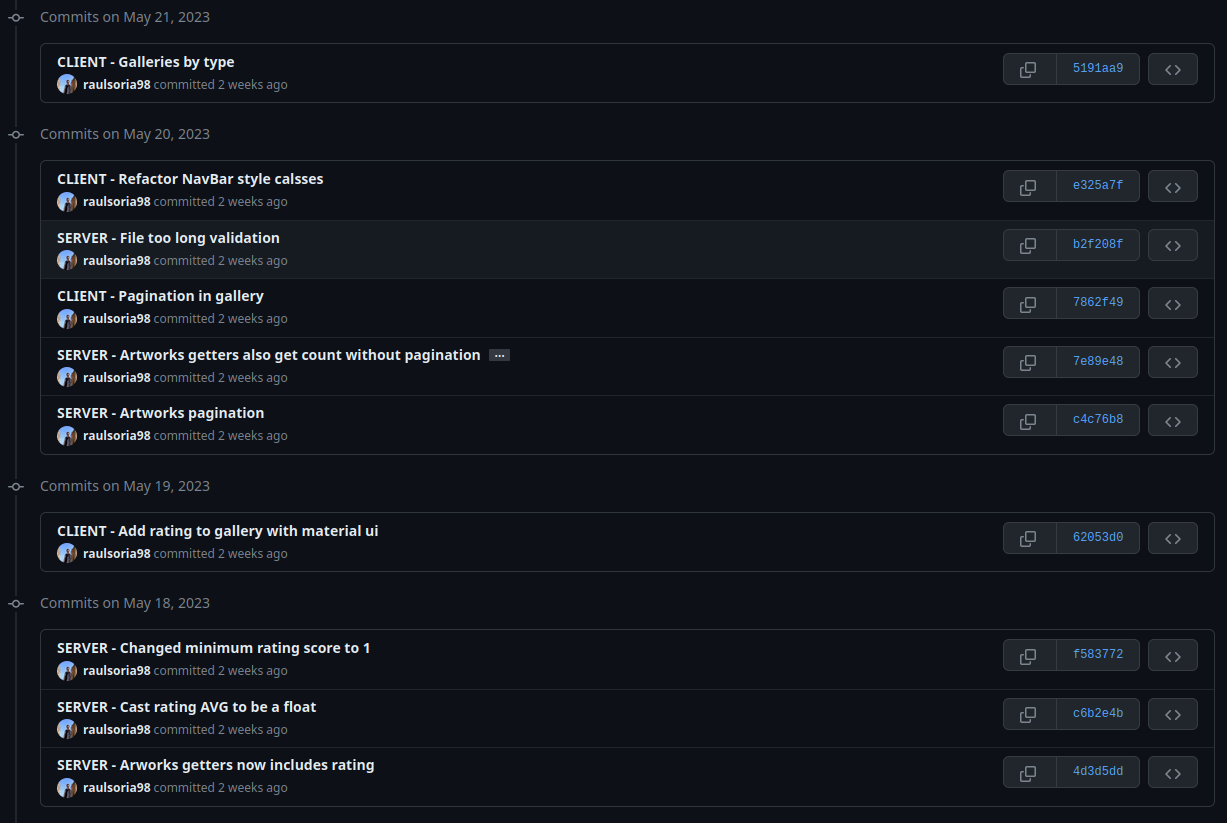
\includegraphics[width=1\textwidth]{commits}
  \caption{Ejemplo de mensajes de commit}
  \label{fig:commits}
\end{figure}

\subsection{Base de datos}
Para la base de datos había que elegir en primer lugar entre una base de datos
relacional o una base de datos no relacional.

En este artículo \cite{relational-vs-non-relational} se explica la diferencia entre
un tipo de base de datos y otro, las ventajas que tiene cada una y en qué casos es
más recomendable utilizar una u otra.

En el caso de nuestra aplicación, se ha optado por utilizar una base de datos relacional
ya que, aunque la base de datos no va a ser muy grande, sí que va a tener una estructura
bien definida con relaciones fuertes entre las tablas.

También es necesario elegir el gestor de base de datos que se va a utilizar, ya que
existen varios gestore de bases de datos relacionales. En nuestro caso se ha optado
por utilizar \textit{MySQL} \cite{mysql} ya que es el gestor de bases de datos
relacionales más utilizado y es el que más conozco personalmente.

\subsection{Backend}
Para el desarrollo del backend de la aplicación se ha utilizado \textit{Node.js}
\cite{nodejs} que es un entorno de ejecución de JavaScript. Se ha elegido este
entorno porque quería aprender a utilizarlo dada su popularidad y porque así podría
utilizar JavaScript tanto en el backend como en el frontend. Este último punto
hizo que descartara utilizar otros frameworks como \textit{Django} \cite{django}
o \textit{Ruby on Rails} \cite{ruby-on-rails}.

Como framework complementario a \textit{Node.js} se ha utilizado \textit{Express}
\cite{express} que facilita la creación de aplicaciones web y de APIs en \textit{Node.js}.

\subsection{Frontend}
Para el desarrollo del frontend de la aplicación se barajaron varias opciones.
En primer lugar, se pensó en utilizar \textit{Angular} \cite{angular} ya que es un
framework bastante popular y con el que ya había trabajado anteriormente. Sin embargo,
se descartó esta opción porque, como explican en este artículo \cite{angular-vs-react},
este es un framework muy completo y pensado para aplicaciones grandes donde prima el
trabajo en equipo ya que su estructura es fija y la esto la hace más compleja. Mientras
que \textit{React} \cite{react} es una librería más sencilla y flexible que permite
crear aplicaciones pequeñas como la nuestra de manera sencilla y sin una gran curva de
aprendizaje.

También se barajó la opción de utilizar \textit{Vue.js} \cite{vuejs} ya que es una
librería de la que también había oído hablar y que también usa JavaScript.
Como comentan en este otro artículo \cite{vuejs-vs-react}, \textit{Vue.js} \cite{vuejs}
también es una librería bastante sencilla y ligera, cuyos módulos se pueden ir añadiendo
según se vayan necesitando. Sin embargo, se descartó esta opción porque, aunque
\textit{Vue.js} \cite{vuejs} es más sencillo que \textit{React} \cite{react}, este
último tiene mayor rendimiento, además, me llamaba más la atención y quería aprender a
utilizarlo.


\section{Implementación de la base de datos}
Para la implementación de la base de datos \textit{MySQL} \cite{mysql} se ha utilizado
\textit{Sequelize} \cite{sequelize} que es un ORM (Object-Relational Mapping) para
\textit{Node.js} \cite{nodejs} que permite trabajar con bases de datos relacionales
como la que se ha utilizado en este proyecto.

Tal y como se explica en este artículo \cite{orm} \textit{'Un ORM (Object Relational
Mapping o Mapeo Objeto-Relacional en castellano) es una herramienta que nos permite mapear, o lo
que es lo mismo, convertir los objetos de tu aplicación a un formato adecuado para ser
almacenados en cualquier base de datos, creándo para ello una base de datos virtual
donde los datos disponibles en nuestra aplicación quedan vinculados con la base de datos
final.'}

Con \textit{Sequelize} \cite{sequelize} se define la conexión a la base de datos como se
puede ver en el código de la imágen \ref{fig:sequelize-db} correspondiente al archivo
\texttt{config/db.js}. Creando un objeto \texttt{sequelize} que servirá para,
posteriormente, realizar la conexión o definir los modelos de la base de datos. Como se
puede ver, el nombre de la base de datos, el usuario, la contraseña, el host y el puerto
se han definido en variables de entorno en un archivo \texttt{.env} para que no se vean
reflejados en el código fuente y así evitar que se suban a \textit{GitHub} \cite{github}.

\begin{figure}[H]
  \centering
  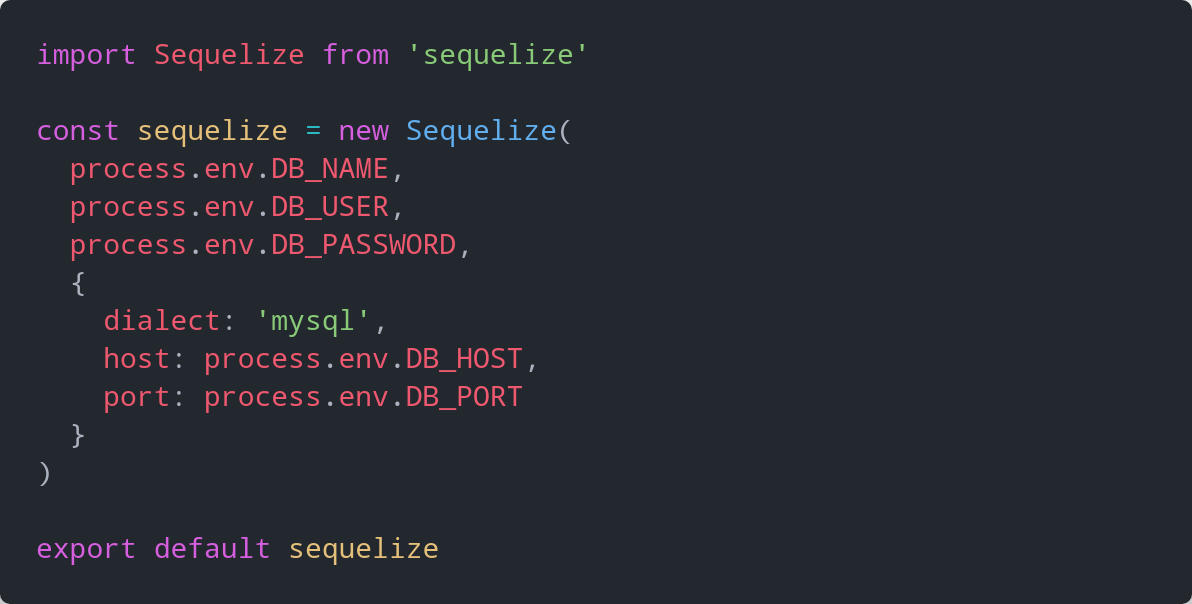
\includegraphics[width=1\textwidth]{img/sequelize-db}
  \caption{Definición de la conexión a la base de datos con \textit{Sequelize}}
  \label{fig:sequelize-db}
\end{figure}

Una vez definida la conexión a la base de datos, se realiza la conexión con la misma
mediante el método \texttt{authenticate()} como se puede ver en el código de la imágen
\ref{fig:sequelize-connect} donde se define una función de conexión que se ejecuta
cuando se inicia la aplicación.

\begin{figure}[H]
  \centering
  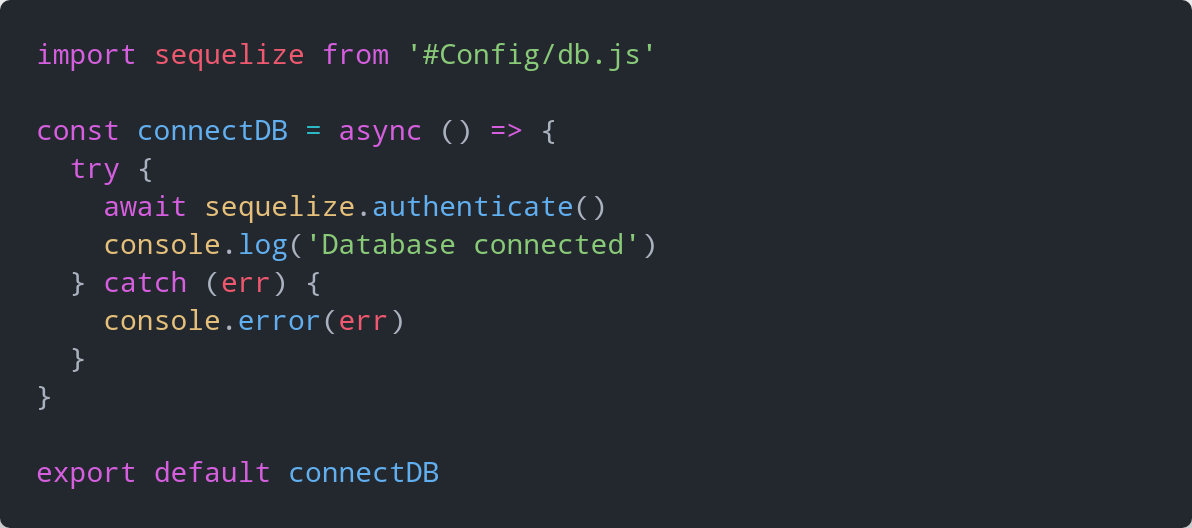
\includegraphics[width=1\textwidth]{img/sequelize-connect}
  \caption{Conexión a la base de datos con \textit{Sequelize}}
  \label{fig:sequelize-connect}
\end{figure}

Para la definición de los modelos de la base de datos se ha seguido la documentación
de \textit{Sequelize} \cite{sequelize-models} donde se explica cómo definir los modelos.
En la aplicación se han creado los archivos correspondientes
a cada modelo. Como por ejemplo el archivo \texttt{artwork.js}, cuyo código se puede ver
en la imágen \ref{fig:artwork-model}, donde se define el modelo \texttt{Artwork} con sus
atributos, validaciones y constraints.

\begin{figure}[H]
  \centering
  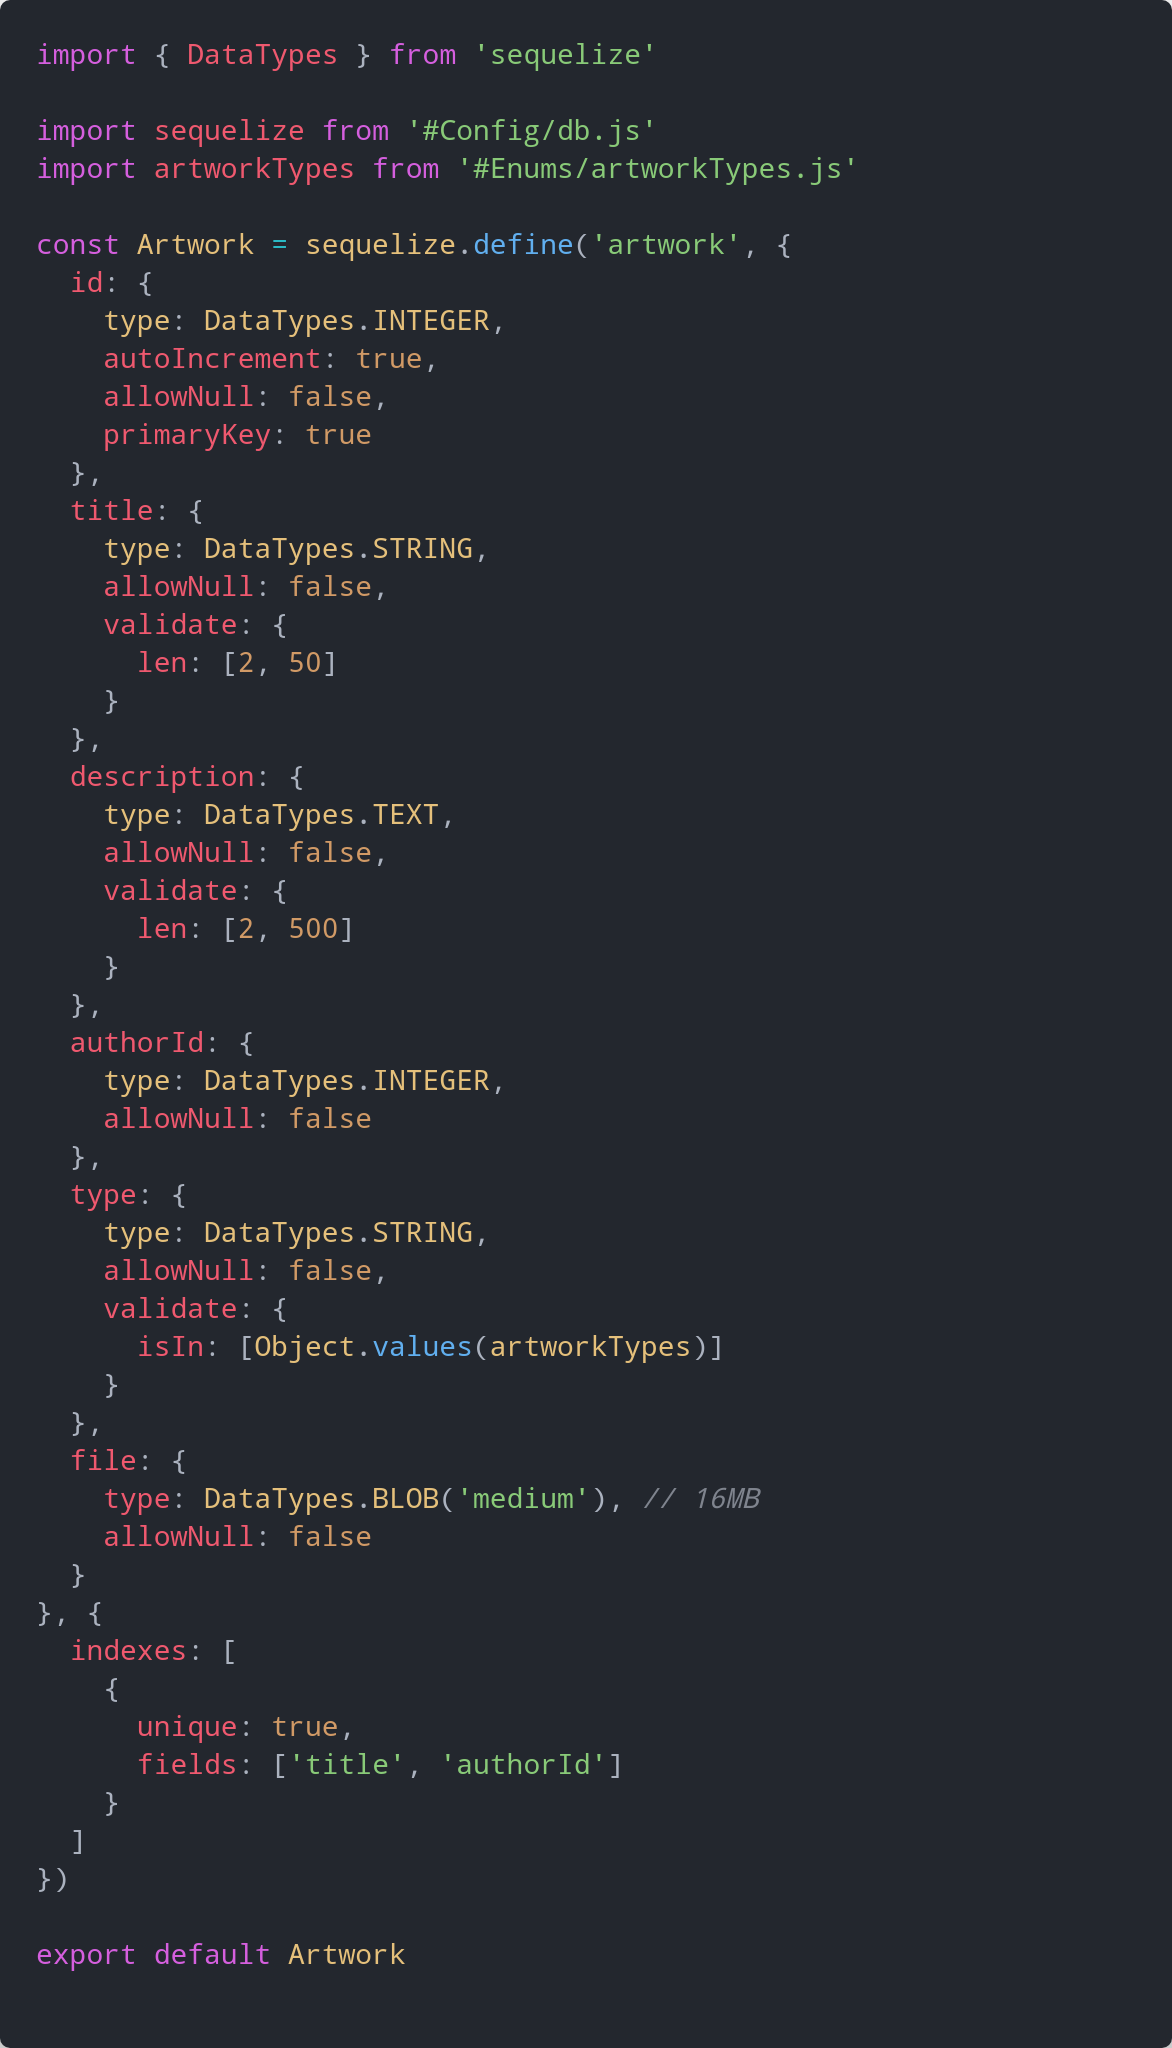
\includegraphics[width=0.8\textwidth]{img/artwork-model}
  \caption{Definición del modelo \texttt{Artwork}}
  \label{fig:artwork-model}
\end{figure}

Para las relaciones entre los distintos modelos se han seguido las instrucciones
de la documentación oficial \cite{sequelize-associations}. Se definen en una función
\texttt{associateModels} que se ejecuta justo después de realizar la conexión a la base
de datos. Como se puede ver en el código de la imágen \ref{fig:associate-models}, se
define la relación uno a muchos entre el modelo \texttt{User} y el modelo \texttt{Artwork},
la relación uno a uno entre el modelo \texttt{User} y el modelo \texttt{Rating} y la
relación uno a muchos entre el modelo \texttt{Artwork} y el modelo \texttt{Rating}.

También se puede ver que se definen las claves externas de cada relación y un alias para
cada una de ellas. Esto permite realizar consultas que incluyan datos de los modelos
relacionados de manera más sencilla.

\begin{figure}[H]
  \centering
  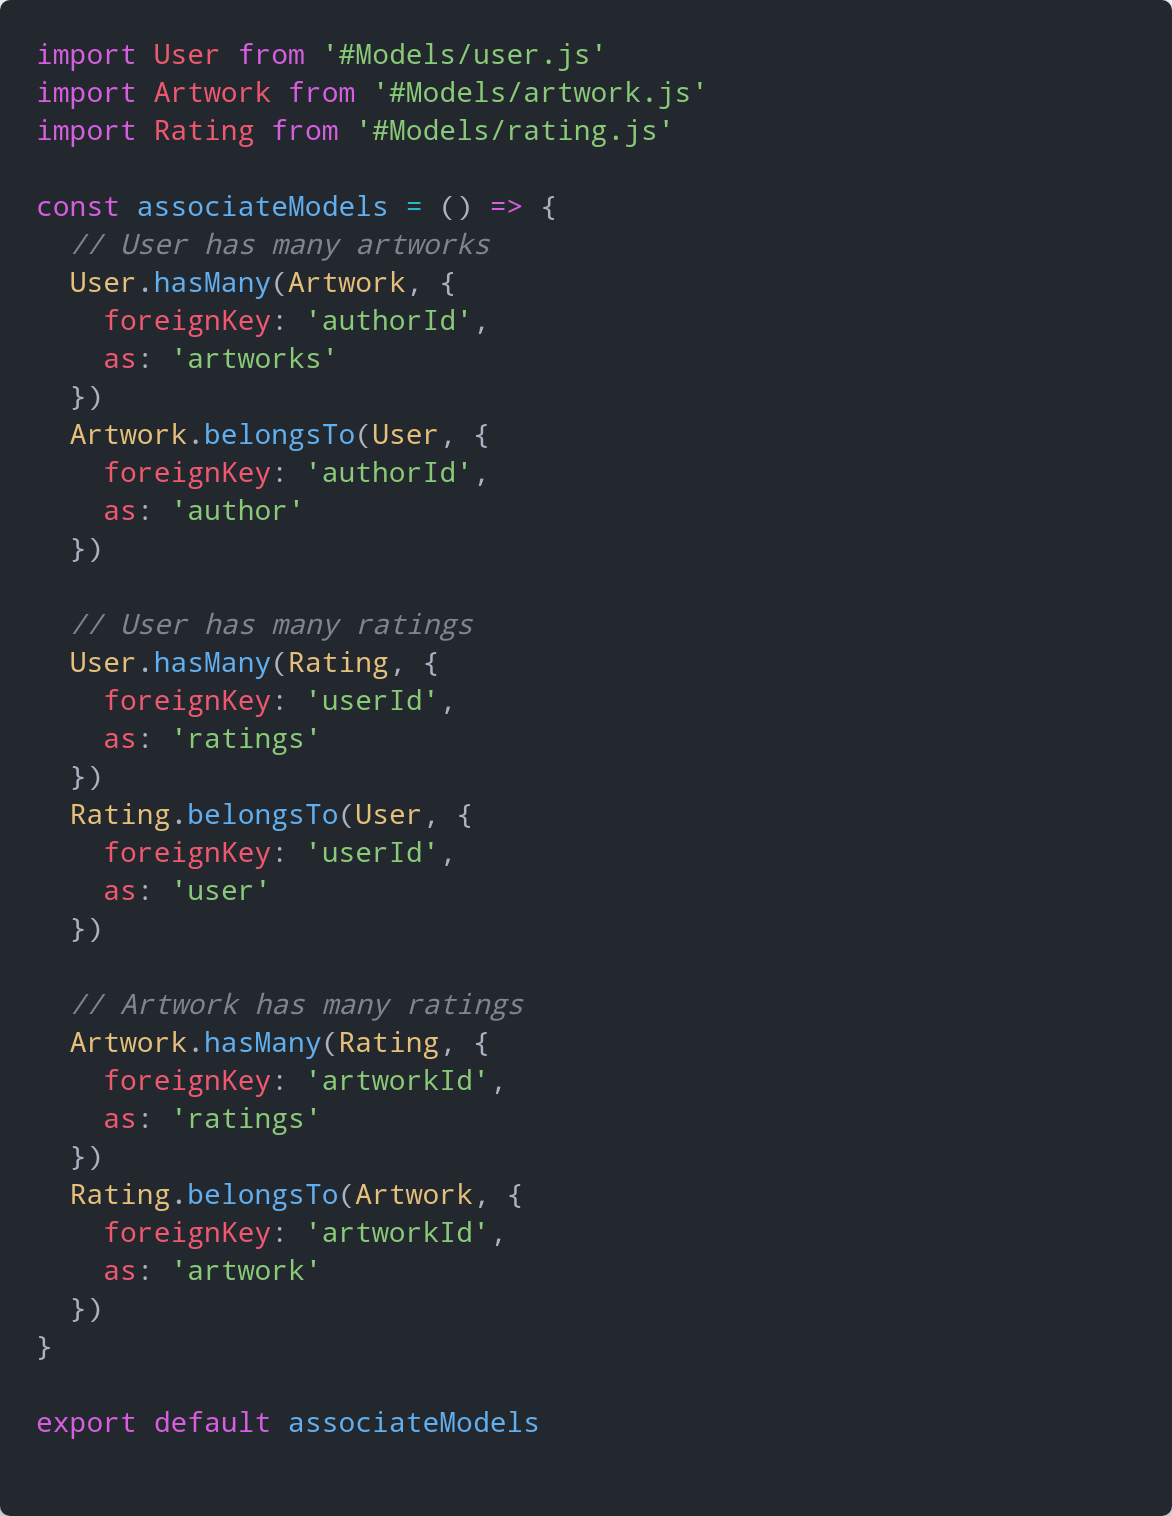
\includegraphics[width=1\textwidth]{img/associate-models}
  \caption{Definición de las relaciones entre los modelos}
  \label{fig:associate-models}
\end{figure}

Para la gestión de la base de datos se ha utilizado \textit{PhpMyAdmin} \cite{phpmyadmin}
que es una herramienta de administración de bases de datos basada en web, ofreciendo una
interfaz gráfica desde la que poder ver y gestionar los datos de la aplicación por parte
de los administradores.

\section{Diagrama de clases}

\section{Implementación de la aplicación}
